\documentclass[12pt,a4paper,titlepage]{report}
\usepackage[utf8]{inputenc}
\usepackage[german,english]{babel}
\usepackage[T1]{fontenc}
\usepackage{lmodern}
\usepackage{amsmath}
\usepackage{amsfonts}
\usepackage{amssymb}
\usepackage[left=2cm,right=2cm,top=2cm,bottom=2cm]{geometry}
\usepackage[]{hyperref}
\hypersetup{
	colorlinks,
	linkcolor = blue
}
\usepackage{graphicx}
\usepackage{svg}
\usepackage{float}
%%Source code listings:
\usepackage{listingsutf8}
\usepackage{color}
\definecolor{mygreen}{rgb}{0,0.6,0}
\definecolor{mygray}{rgb}{0.5,0.5,0.5}
\definecolor{mymauve}{rgb}{0.58,0,0.82}
\lstset{
  backgroundcolor=\color{white},   % choose the background color; you must add \usepackage{color}
  basicstyle=\footnotesize,        % the size of the fonts that are used for the code
  breakatwhitespace=false,         % sets if automatic breaks should only happen at whitespace
  breaklines=true,                 % sets automatic line breaking
  captionpos=b,                    % sets the caption-position to bottom
  commentstyle=\color{mygreen},    % comment style
  deletekeywords={...},            % if you want to delete keywords from the given language
  escapeinside={\%*}{*)},          % if you want to add LaTeX within your code
  extendedchars=true,              % lets you use non-ASCII characters; for 8-bits encodings only, does not work with UTF-8
  frame=single,	                   % adds a frame around the code
  keepspaces=true,                 % keeps spaces in text, useful for keeping indentation of code (possibly needs columns=flexible)
  keywordstyle=\color{blue},       % keyword style
  language=PHP,                    % the language of the code
  morekeywords={*,...},            % if you want to add more keywords to the set
  numbers=left,                    % where to put the line-numbers; possible values are (none, left, right)
  numbersep=5pt,                   % how far the line-numbers are from the code
  numberstyle=\tiny\color{mygray}, % the style that is used for the line-numbers
  rulecolor=\color{black},         % if not set, the frame-color may be changed on line-breaks within not-black text (e.g. comments (green here))
  showspaces=false,                % show spaces everywhere adding particular underscores; it overrides 'showstringspaces'
  showstringspaces=false,          % underline spaces within strings only
  showtabs=false,                  % show tabs within strings adding particular underscores
  stepnumber=1,                    % the step between two line-numbers. If it's 1, each line will be numbered
  stringstyle=\color{mymauve},     % string literal style
  tabsize=4,	                   % sets default tabsize to 2 spaces
  title=\lstname                   % show the filename of files included with \lstinputlisting; also try caption instead of title
}
%% Drawing Keyboard keys:
\usepackage[os=win]{menukeys}
\renewmenumacro{\directory}{pathswithfolder} % default: paths
\renewmenumacro{\keys}{shadowedangularkeys} % default: roundedkeys


\author{Martin Mandelkow}
\title{pharmacy duty roster\\Documentation}

\begin{document}
\maketitle
\tableofcontents


\chapter{Introduction}
Pharmacy Duty Roster (PDR) is a web application that allows to operate a duty roster for pharmacies.
PDR started in 2015 as an alternative to a really simple excel sheet without formulas.
PDR aims to be user-friendly but at the same time cover all necessary features.
PDR continuously strives to improve. It is open to your requests and wishes.
I hope it will fulfil your expectations.
\section{Getting PDR}
The latest release of PDR is available on \href{https://github.com/MaMaKow/dienstplan-apotheke/releases/latest}{GitHub}. GitHub provides the source code as *.zip file or *.tar.gz ball. Extract the files into a folder.

Make sure to unpack PDR to a directory, that your webserver has access to. PHP and the webserver must have read access to all the files and folders. It also needs write access to the subdirectories upload, tmp and config. You might want to change the owner of the directory to the webservers user with e.g.:

You can also clone the repository with git:
\begin{verse}
git clone https://github.com/MaMaKow/dienstplan-apotheke.git
\end{verse}
See the Administrator manual for details!

\section{License}
PDR is open source software under the AGPL license.
\begin{quote}
	Copyright (C) 2018  Dr. Martin Mandelkow
	
	This program is free software: you can redistribute it and/or modify
	it under the terms of the GNU Affero General Public License as
	published by the Free Software Foundation, either version 3 of the
	License, or (at your option) any later version.
	
	This program is distributed in the hope that it will be useful,
	but WITHOUT ANY WARRANTY; without even the implied warranty of
	MERCHANTABILITY or FITNESS FOR A PARTICULAR PURPOSE.  See the
	GNU Affero General Public License for more details.
	
	You should have received a copy of the GNU Affero General Public License
	along with this program.  If not, see <https://www.gnu.org/licenses/>.
	
\end{quote}
 Please see the \href{https://github.com/MaMaKow/dienstplan-apotheke/blob/master/LICENSE.md}{license file} for details!
\section{Reporting bugs}
The issue tracker is currently located at GitHub.
GitHub requires an account in order to report bugs or feature requests. If you do not want to create one, you might send a mail to pdr-issues@martin-mandelkow.de
\section{How to contribute}
Pull requests are desired. If you made changes to PDR and want to contribute them to the public, you are welcome to open a pull-request on GitHub or send your changes in any other way.


\chapter{User manual}


\section{The web interface}
You can connect to your PDR instance using any web browser. Just navigate to your server and enter your username and password.

\subsection{Login}
\begin{figure}[h]
	\centering
	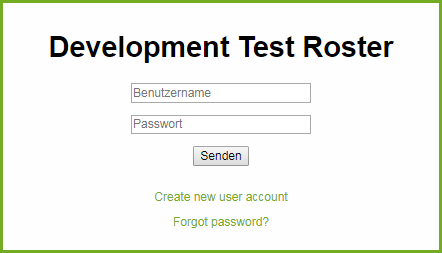
\includegraphics[width=.3\linewidth]{{images/en_GB/login.php}.png}
	\caption{Login page}
\end{figure}
The login page shows the name of the application. You are prompted to enter your username and password.
If you do not have an account yet, you can \menu{Create a new user account}.
If you have an account, but forgot about your password, or want to change it, you can click on \menu{Forgot password?}.


\subsection{Create new user account}
\begin{figure}[ph]
	\centering
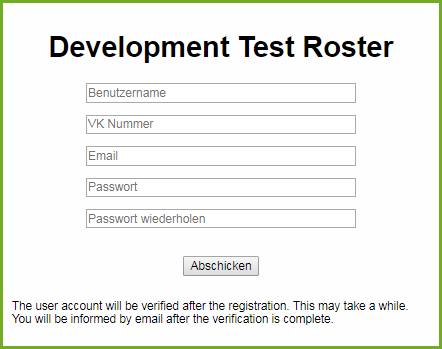
\includegraphics[width=0.4\linewidth]{{images/en_GB/register.php}.png}
	\caption{Register new user page}
\end{figure}
Choose a user name, enter your employee id and your email. Pick a secure password.

The account will be inactive until an administrator activates it. The main administrator is informed via email regarding the registration.

New users can only be created for existing employees. New employees are created by an administrator. 

\subsection{Lost password}
\begin{figure}[h]
    \centering
    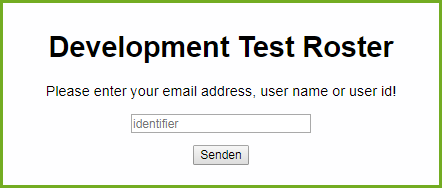
\includegraphics[width=.3\linewidth]{{images/en_GB/lost_password.php}.png}
    \caption{Lost password page}
\end{figure}
The lost password page shows the name of the application. You are prompted to enter either your username, id or your email-address at your option.
After you submit the form, an email is sent to your stored email address.
In that email you will find a link, which will lead you to the password change page.
\subsubsection{Lost password recovery}
\begin{figure}[ph]
    \centering
    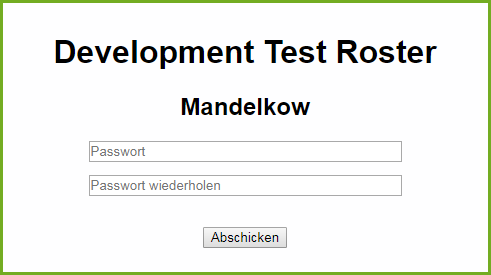
\includegraphics[width=0.3\linewidth]{{images/en_GB/reset-lost-password.php}.png}
    \caption{Lost password recovery page}
\end{figure}
The lost password recovery page shows the name of the application and your user name. You are prompted to enter a new password twice.


\subsection{Navigation}
\begin{figure}[ph]
	\centering
	
\includegraphics[width=0.8\linewidth]{{images/en_GB/navigation}.png}
	\caption{Navigation bar}
	\label{img_navigation_bar}
\end{figure}
By default, the PDR web interface opens a menu containing 5 tiles.
You can navigate to:
\begin{itemize}
\item Roster week table view 
\includegraphics[height=2em]{../img/week_2}
\item Roster daily view 
\includegraphics[height=2em]{../img/day}
\item Roster employee view 
\includegraphics[height=2em]{../img/employee_2}
\item Overtime  
\includegraphics[height=2em]{../img/watch_overtime}
\item Absence 
\includegraphics[height=2em]{../img/absence}
\end{itemize}

\subsubsection{The navigation bar}
In the top there is a navigation bar containing hyperlinks to nearly all the pages of PDR. Hover the mouse over an entry to open the submenus (Figure \ref{img_navigation_bar}).
\begin{multicols}{3}
\begin{description}
    \item \menu{Weekly view > .. }
    \begin{description}
        \item \menu{.. > Weekly table}
        \item \menu{.. > Weekly images}
    \end{description}
    \item \menu{Daily view > .. }
    \begin{description}
    \item \menu{.. > Daily input}
    \item \menu{.. > Daily output}
    \item \menu{.. > Principle roster daily}
    \end{description}
    \columnbreak
    \item \menu{Employee > .. }
    \begin{description}
    \item \menu{.. > Roster employee}
    \item \menu{.. > Principle roster employee}
    \end{description}
    \item \menu{Overtime > ..}
    \begin{description}
    \item \menu{.. > Overtime input}
    \item \menu{.. > Overtime output}
    \item \menu{.. > Overtime overview}
    \end{description}
    \item \menu{Absence > ..}
    \begin{description}
    \item \menu{.. > Absence input}
    \item \menu{.. > Absence annual plan}
    \item \menu{.. > Absence monthly plan}
    \end{description}
    \columnbreak
    \item \menu{Administration > ..}
    \begin{description}
    \item \menu{.. > Attendance list}
    \item \menu{.. > Saturday list}
    \item \menu{.. > Marginal employment hours list}
    \item \menu{.. > Upload deployment planning}
    \item \menu{.. > Human resource managament}
    \item \menu{.. > Branch managament}
    \item \menu{.. > User managament}
    \item \menu{.. > Configuration}
    \item \menu{.. > phpMyAdmin}
    \end{description}
\end{description}
\end{multicols}
\subsection{Roster week table view}
\begin{figure}[h]
	\centering
	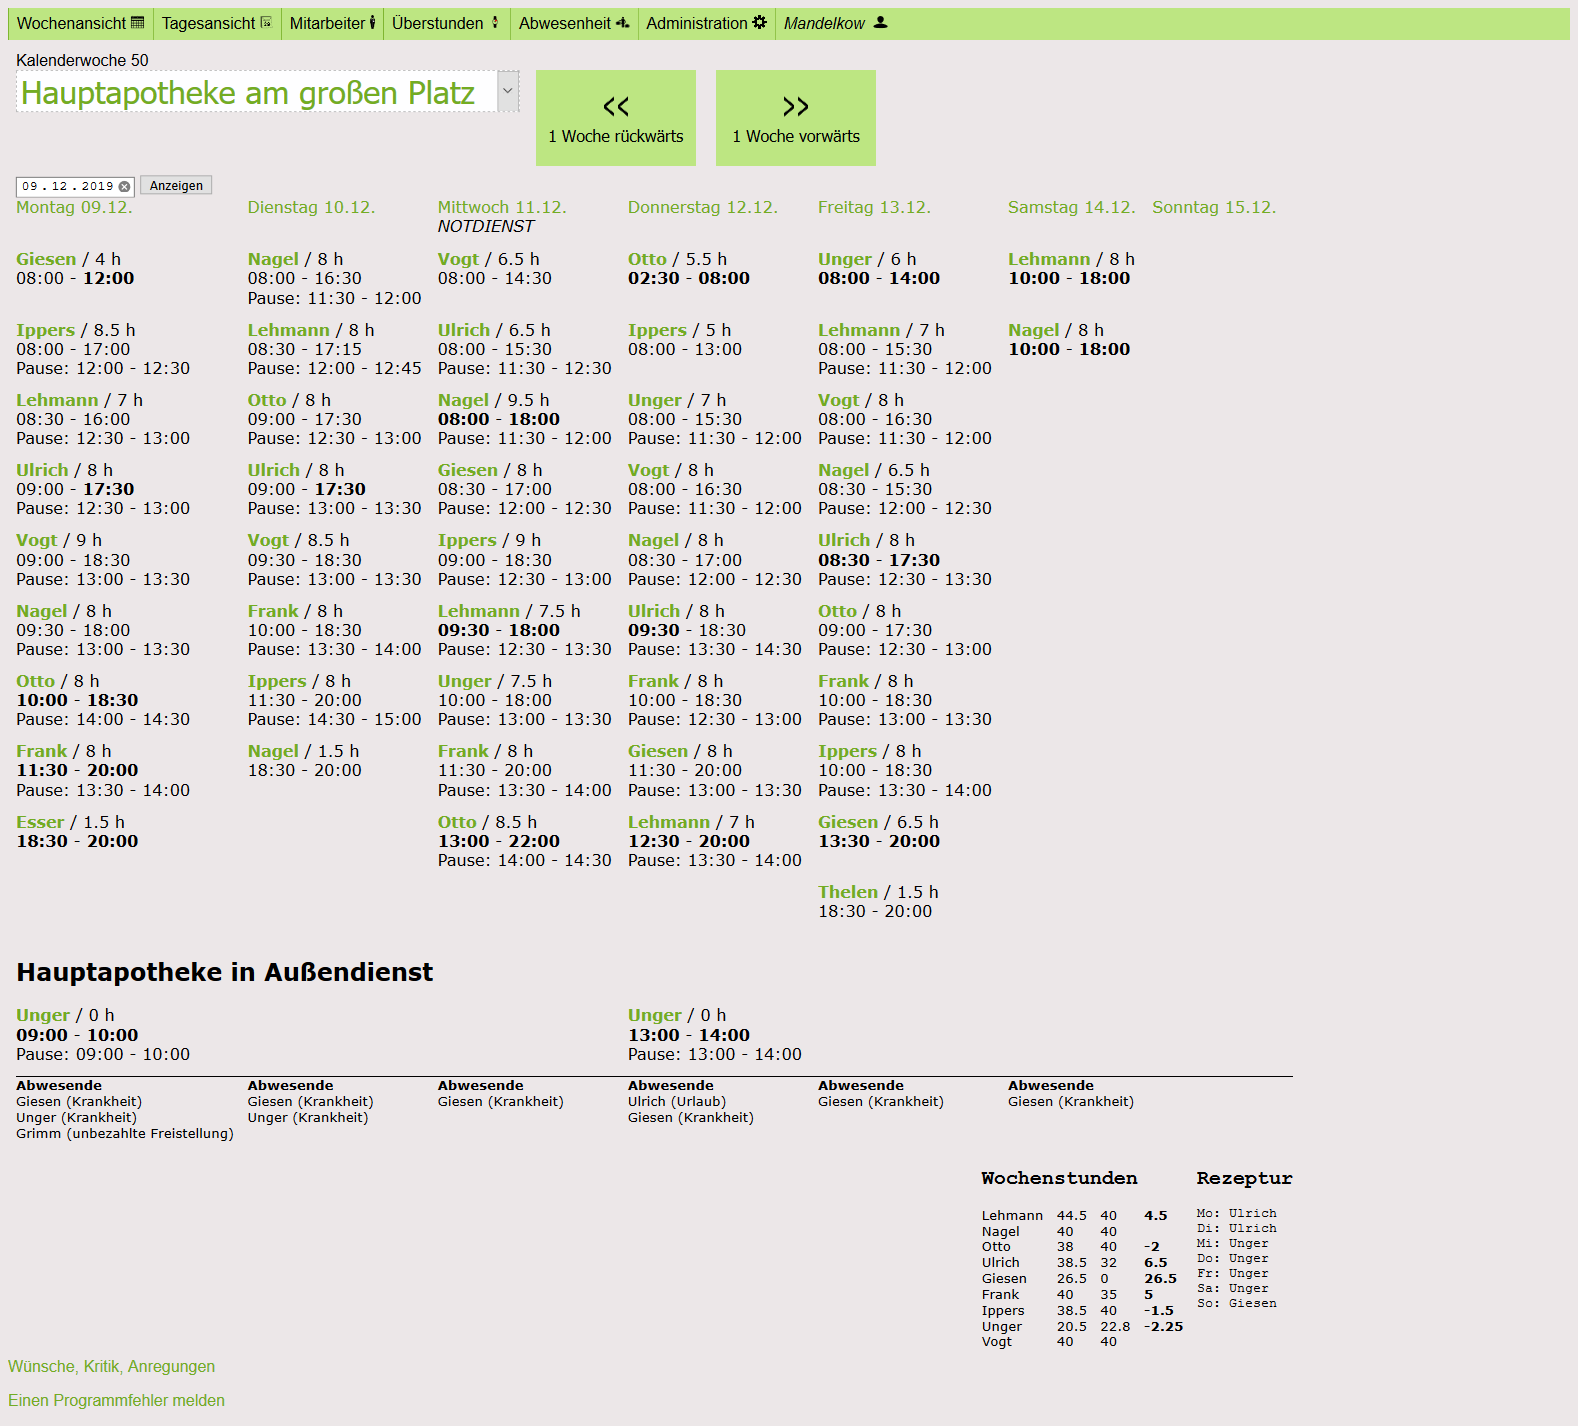
\includegraphics[width=0.8\linewidth]{{images/en_GB/roster-week-table.php}.png}
	\caption{Roster week table view, excerpt without task rotation and weekly working hours}
	\label{img_roster_week_table_view}
\end{figure}

The roster week table view shows the roster of a chosen week an a chosen branch (Figure \ref{img_roster_week_table_view}). If employees of the branch are working in an other branch, then those are shown below.
The table foot contains the information about absent employees and their reason of absence.

The date can be chosen by direct input. It can also be shifted by one week backwards or forwards by pressing \keys{\ctrl + \shift + $\rightarrow$} or \keys{\ctrl + \shift + $\leftarrow$} respectively.

\subsection{Roster daily view}
\subsubsection{Read only}
In the daily roster view there is a table, a bar plot and a histogram reflecting the roster.
The roster table lists all the employees scheduled in the chosen branch on the one chosen day. For every entry there is the employee id and last name, the working hours, the start and end of duty and the time of the lunch break, if any.

If an employee, that is primarily scheduled in the chosen branch, works in an other branch, then this entry is shown in the table at the bottom.
An employee may have more than one entrie per day. This allows divided working time to be stored.
If employees are absent, these absences are displayed in the table footer.


The roster bar plot shows the flow of employees coming and going. Each bar represents one entry. It reaches from the start of duty to its end. A white rectangle on the bar shows the time of the lunch break. The color of the bars is dependent on the profession of the employee. Pharmacists and Pharmazieingenieure \footnote{specific eastern german profession, see \url{https://de.wikipedia.org/wiki/Pharmazieingenieur}} are colored in dark green, while Pharmacy technicians are colored in light green. Other employees (non-pharmaceutical personnel) are colored in grey.

The histogram plot shows a red area and a green line. The red area shows the expected amount of work (measured in packages per 15 minutes), while the green line represents the amount of working employees to any given time.


\subsubsection{Edit}
The edit page looks quite similar to the read only view. 
The roster is examined for errors. If any issues occur, then errors, warnings or information will be shown in the top right area.
The examination includes:
\begin{itemize}
    \item overlap of shifts for the same employee (Error)
    \item sufficient employee count (Warning, hardcoded at least two employees)
    \item attendence of at least one pharmacist at any time (Error).
    \item attendance of at least one person able to carry out goods receipt (Warning).
    \item scheduling of absent employees (Error)
    \item non-scheduling of non-absent employees (Warning)
\end{itemize}

Only one break can be inserted per entry. If more breaks have to be assigned, then it is possible to enter multiple entries for the same employee.
\subsection{Roster employee view}
\subsection{Overtime}
\subsection{Absence}
There are four views to the absence data.
\begin{itemize}
\item Employee view readonly
\item Employee view edit
\item Monthly table
\item Year overview
\end{itemize}
In the \emph{Employee view readonly} there is a select element to choose the employee to view. There is a button to switch to the edit view.
And there is a table containing the absence data. The columns are start and end of the absence, reason of absence and number of days.
There is a distinct list of possible reasons ( vacation,
        remaining holiday,
       sickness,
        sickness of child,
        unpaid leave of absence,
        paid leave of absence,
        parental leave and
        maternity leave).
The number of days of absence is calculated for a 5 day week. Absences on saturdays and sundays are registered but not counted. The same applys for holidays.
\chapter{Administrator manual}
\section{Installation}\label{sec:installation}
\subsection{Getting PDR}
\subsection{The installer}
\subsubsection{Introduction}
The first page shows some non-technical information about this program. Click \menu{Next} to move on!
\subsubsection{Welcome}
On the second page some technical background information is given. You are informed about the necessary input information, required for continuing the installation. Available database management systems (currently only MySQL) are listed. Finally, you are informed about the user and password strategy for the database access. Click \menu{Next} again, to continue.
\subsubsection{Requirements}
On the next page the application checks, if all requirements are met. The requirements include a minimum PHP version, some PHP extensions and support for database connections. Also the program needs write access to some of its directories.
If problems are found, then a descriptive error message will be shown. It is not possible to continue, until all problems are solved.
Click \menu{Next} again, to continue.
\subsubsection{Database configuration}
The application now starts to collect configuration data.
\begin{itemize}
\item Database type
\item hostname
\item port (optional)
\item username \\An existing database user. The user MUST have the privilege to create a database. The user SHOULD have the privilege to create a less privileged user.
\item password \\The database password of the user. If a new user could be created, then a new secure random password will be given to the new user.
\item database name
\end{itemize}
\subsection{First steps}
\section{Upgrading}
\section{Configuration}
\section{Maintenance}
\section{Issues and Troubleshooting}



\chapter{Developer manual}


\section{Core development}
All PHP scripts have a common file \texttt{default.php}, which handles the default settings. It is placed at ./, which is the \texttt{PDR\_FILE\_SYSTEM\_APPLICATION\_PATH}.
See the file below:
\lstinputlisting[language=PHP]{../default.php}

\subsection{Directory structure}
\begin{itemize}
\item \directory{config/} Contains the configuration file config.php
\item \directory{css/} \emph{obsolete}, use \directory{src/css/} instead
\item \directory{docs/} This documentation and tools to build it
\item \directory{img/} Images used by the program
\item \directory{js/}  \emph{obsolete}, use \directory{src/js/} instead
\item \directory{locale/} translation files for gettext, currently only german (de\_DE)
\item \directory{src/} Most of the actual source code
    \begin{itemize}
    \item \directory{src/css} Style Sheets
    \item \directory{src/js} JavasScript
    \item \directory{src/php/} PHP: Hypertext Preprocessor
    \item \directory{src/php/classes/} Contains all the class files class.class\_name.php
    \item \directory{src/php/fragments/} parts of bigger pages, may be included via php require/include or loaded with JavaScript
    \item \directory{\textbf{src/php/pages/}} This is the place for the single views, which the human user will use to look at the roster etc.
    \item \directory{src/sql/} SQL Database Tables and Triggers
    \end{itemize}
\item \directory{tests/} Tests to find errors in the source code; This folder is listed in .gitignore. Only some files are part of the visible source.
\item \directory{tmp/} A directory for temporary files. There is no automatic cleanup yet.
\item \directory{upload/} The destination for uploaded content. Currently only specific *.PEP files produced by Awinta ASYS Smart are understood. Those files contain information about the amount of customers that have been served in the past.
\end{itemize}

\subsection{Coding standards}
This project aims to follow some coding style guide.
\begin{itemize}
\item Please avoid StudlyCaps and camelCase.
\item Class constants MUST be declared in all upper case with underscore separators.
\item Property names MUST be written in under{\_}score.
\item Plain variables and objects are written in all lowercase.
\item Array names start with a singe Uppercase letter followed by lowercase characters.
\item Method names MUST be written in under{\_}score.

\item Code MUST use 4 spaces for indenting, not tabs.
\item Opening braces for classes and functions MUST go on the same line, and closing braces MUST go on the next line after the body.
\item Opening braces for control structures SHOULD go on the same line, and closing
braces MUST go on the next line after the body.
\end{itemize}
Disk space is not rare anymore. IDEs are helping with autocomplete. There is no need to abbreviate stuff. Please use long terms like \lstinline|user_email_notification_cache| instead of \lstinline|usr_ml_ntfcn_ca| or \lstinline|u_e_n_c|. 

\subsection{The database}
Currently there is only MySQL supported as a database management system (DBMS).
The tables are:
\begin{itemize}
\item absence (illness, vacation and other kinds of absence)
\item approval (saves for each day if the leader has officially authorized the roster)
\item branch (information about the main pharmacy and possible branches)
\item Dienstplan (the actual roster data; start, end, break)
\item employees (employee data; employee\_id, name, profession, abilities)
\item employees\_backup (a copy of the employees table with historical data archived)
\item Feiertage (obsolete)
\item principle\_roster (the basic plan; start, end, lunch break; is used to suggest new rosters)
\item maintenance (obsolete)
\item Mandant (obsolete)
\item Notdienst (dates of emergency services and the employees scheduled to them)
\item opening\_times\_special (not used yet)
\item opening\_times (the opening and closing times of the branches, no GUI yet for editing)
\item pdr\_self (reflects the state of the application itself)
\item pep\_month\_day (the relative amount of work on different days in the month)
\item pep (the raw amount of work data, hashed to reduce the amount of deleted/ignored entries)
\item pep\_weekday\_time (the amount of work at different times on different weekdays)
\item pep\_year\_month (the relative amount of work on different months in the year)
\item saturday\_rotation (whose turn is it to work on which saturday?)
\item saturday\_rotation\_teams (who belongs to which team for saturday's rotation?)
\item Schulferien (not used yet)
\item Stunden (overtime archive and balance)
\item task\_rotation (rotating assignment of employees to a task, e.g. compounding)
\item user\_email\_notification\_cache (not used yet)
\item users\_lost\_password\_token (tokens provided to change a forgotten password)
\item users\_privileges (the privileges of the user accounts)
\item users (the user accounts; there has to be exacly one employee for every user account; there may be employees without user accounts)
\item Wunschplan (obsolete)
\end{itemize}


A copy of all the table structures is stored in \directory{src/sql/}.
The directory also contains the file \directory{src/sql/database\_version\_hash.php} which holds a SHA1 hash of all 
the structures returned by \lstinline|SHOW CREATE TABLE| and \lstinline|SHOW CREATE TRIGGER| after some modification. 
The hash is written by \directory{tests/get-database-structure.php}, see the details in that file.

\subsubsection{Maintenance of the database}
There is a class \emph{update\_database}.
This class holds a defined set of MySQL statements that alter the database structure from a known state in the past to the current state.

This class is not well tested. It might work. It might as well destroy the whole database.

The class \emph{update\_database} is called on every login of a user. It then decides on its own, if any actions have to be taken.
In order to decide, the hash stored in the file \directory{database\_version\_hash.php} is compared to the hash stored in the database table \menu{pdr\_self > pdr\_database\_version\_hash}.

\paragraph{Auto healing tables}
The class \emph{database\_wrapper} has a function \emph{create\_table\_from\_template()} that is able to create missing tables from the structure information given in \directory{src/sql/}. It is called if any PDO database query throws an exception with the code 42S02 and the MySQL error 1146.

\subsection{Classes}
The classes are stored in the folder \directory{src/php/classes/} or \directory{src/php/3rdparty/}.
The autoloader will only load classes from \directory{\lstinline|src/php/classes/class.\$class_name.php|}, every other class has to be manually included.

\subsubsection{user}
The user class represents an employee, who has registered a user account in PDR.

\subsubsection{user\_input}
\paragraph{\lstinline|user_input::get_variable_from_any_input|}
This function reads user input from POST, GET or COOKIE in that order.
If the requested information is found in one of the sources, then the others are ignored.
For security reasons all information is filtered. By default \lstinline|FILTER_SANITIZE_STRING| is used. Any other filter can be given as the second parameter.
If no information is found in any of the sources, then a default value (the third parameter) will be returned.

\paragraph{\lstinline|escape_sql_value|} foo
\paragraph{\lstinline|convert_post_empty_to_php_null|} foo
\paragraph{\lstinline|principle_employee_roster_write_user_input_to_database|} foo
\paragraph{\lstinline|principle_roster_write_user_input_to_database|} foo
\paragraph{\lstinline|get_Roster_from_POST_secure|} foo
\paragraph{\lstinline|remove_changed_entries_from_database|} foo
\paragraph{\lstinline|remove_changed_entries_from_database_principle_roster|} foo
\paragraph{\lstinline|insert_changed_entries_into_database_principle_roster|} foo
\paragraph{\lstinline|insert_new_approval_into_database|} foo
\paragraph{\lstinline|old_write_approval_to_database|} foo
\paragraph{\lstinline|get_changed_roster_employee_id_list|} foo
\paragraph{\lstinline|get_deleted_roster_employee_id_list|} foo
\paragraph{\lstinline|get_inserted_roster_employee_id_list|} foo
\paragraph{\lstinline|roster_write_user_input_to_database|} foo






\subsection{Web Interface}

\subsection{Calendar API}
The script does not discriminate between information sent by POST, GET or COOKIE.
See \lstinline|user_input::get_variable_from_any_input| for details.
The parameter \lstinline|date_string| acepts any string that can be interpreted by DateTime
See \url{https://secure.php.net/manual/en/datetime.formats.date.php} for details.


\section{Documentation}
This documentation about a programm, app or script is a stub. You can help this project by expanding it.
Seriously, if there is something that does not explain itself enough, just send me an email or contact me at GitHub!


\section{Testing}


\section{Bug tracker}
Bugs and Issues are tracked at GitHub \url{https://github.com/MaMaKow/dienstplan-apotheke/issues}


\section{Translation}
Translations are handled with gettext().

See this article about po4a about the translation of this document:
\url{https://maltris.org/mehrsprachigkeit-fur-fast-alles-po4a-7317.html}

\subsection{Internationalization}
Different countries have different laws regarding pharmacies and employment. They also have different holidays.

\end{document}
